% Roll Number 61, Swathy M

\textbf{\textcolor{LightMagenta}{With suitable equations, explain any two types of activation functions used in neural networks. (May 2019, Qn 6)\hfill (Mark 6)}} \\[5pt]
ReLu:-
The Rectified Linear Unit (ReLU) function is one of the most popular Activation Functions in Deep Learning models. It is a fast-learning AF that promises to deliver state-of-the-art performance. Compared to other Activation Functions like the sigmoid and tanh functions, the ReLU function offers much better performance and generalization in deep learning. The function is a nearly linear function that retains the properties of linear models, which makes them easy to optimize with gradient-descent methods. The ReLU function performs a threshold operation on each input element where all values less than zero are set to zero. Thus, the ReLU is represented as:
\begin{figure}[htp]
    \centering
    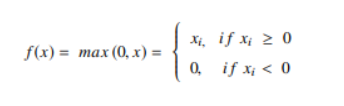
\includegraphics[width=10cm]{Images/A41_img1.png}
 \end{figure}

Softmax: - 
The softmax function is a type of Activation Function used in neural networks to compute probability distribution from a vector of real numbers. This function generates an output that ranges between values 0 and 1 and with the sum of the probabilities being equal to 1. The softmax function is represented as follows:
\begin{figure}[htp]
    \centering
    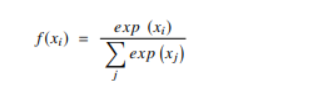
\includegraphics[width=10cm]{Images/A41_img2.png}
 \end{figure}